\documentclass[12pt,letterpaper]{article}
\usepackage[utf8]{inputenc}
\usepackage[spanish]{babel}
\usepackage{graphicx}
\usepackage[left=2cm,right=2cm,top=2cm,bottom=2cm]{geometry}
\usepackage{graphicx} % figuras
% \usepackage{subfigure} % subfiguras
\usepackage{float} % para usar [H]
\usepackage{amsmath}
%\usepackage{txfonts}
\usepackage{stackrel} 
\usepackage{multirow}
\usepackage{enumerate} % enumerados
\renewcommand{\labelitemi}{$-$}
\renewcommand{\labelitemii}{$\cdot$}
% \author{}
% \title{Caratula}
\begin{document}

% Fancy Header and Footer
% \usepackage{fancyhdr}
% \pagestyle{fancy}
% \cfoot{}
% \rfoot{\thepage}
%

% \usepackage[hidelinks]{hyperref} % CREA HYPERVINCULOS EN INDICE

% \author{}
\title{Caratula}

\begin{titlepage}
\begin{center}
\large{UNERSIDAD PRIVADA DE TACNA}\\
\vspace*{-0.025in}
\begin{figure}[htb]
\begin{center}

\includegraphics[width=8cm]{./Imagenes/logo}
\end{center}
\end{figure}
\vspace*{0.15in}
INGENIERIA DE SISTEMAS  \\

\vspace*{0.5in}
\begin{large}
TITULO:\\
\end{large}

\vspace*{0.1in}
\begin{Large}
\textbf{INFORME DE SECTION-FUNDAMENTALS} \\
\end{Large}

\vspace*{0.3in}
\begin{Large}
\textbf{CURSO:} \\
\end{Large}

\vspace*{0.1in}
\begin{large}
BASE DE DATOS II\\
\end{large}

\vspace*{0.3in}
\begin{Large}
\textbf{DOCENTE(ING):} \\
\end{Large}

\vspace*{0.1in}
\begin{large}
 Patrick Cuadros Quiroga\\
\end{large}

\vspace*{0.2in}
\vspace*{0.1in}
\begin{large}
Integrante: \\
\begin{flushleft}
Mamani Limache, Jhony 		\hfill	(2013046566) 
\end{flushleft}
\end{large}
\end{center}

\end{titlepage}


\tableofcontents % INDICE
\thispagestyle{empty} % INDICE SIN NUMERO
\newpage
\setcounter{page}{1} % REINICIAR CONTADOR DE PAGINAS DESPUES DEL INDICE


\include{Secciones/Actividad01}
\include{Secciones/Actividad02}
\section{Actividad No 03 –  Creating PL/SQL Blocks} 
		
\begin{enumerate}[1.]
	\item VOCABULARIO :
	\subitem Identify the vocabulary word for each definition below:
	\subitem 01-\_\_\_\_\_\_\_\_\_\_\_\_\_\_\_\_:Unnamed blocks of code not stored in the database and do not exist after they are executed
	\subitem 02-\_\_\_\_\_\_\_\_\_\_\_\_\_\_\_\_:A program that computes and returns a single value
	\subitem 03-\_\_\_\_\_\_\_\_\_\_\_\_\_\_\_\_:Named PL/SQL blocks that are stored in the database and can be declared as procedures or functions
	\subitem 04-\_\_\_\_\_\_\_\_\_\_\_\_\_\_\_\_:Software that checks and translates programs written in highlevel programming languages into binary code to execute
	\subitem 05-\_\_\_\_\_\_\_\_\_\_\_\_\_\_\_\_:A program that performs an action, but does not have to return a value
	\\\\
	\\01.- CHARACTERISTICS OF ANONYMOUS BLOCKS
	\\02.- FUNCTION
	\\03.- SUBPROGRAMS
	\\04.- C, JAVA, OL/SQL
	\\05.- PROCEDURE

	\item Try It / Solve It
	\subitem 01- Complete the following chart defining the syntactical requirements for a PL/SQL block:
	\begin{center}
	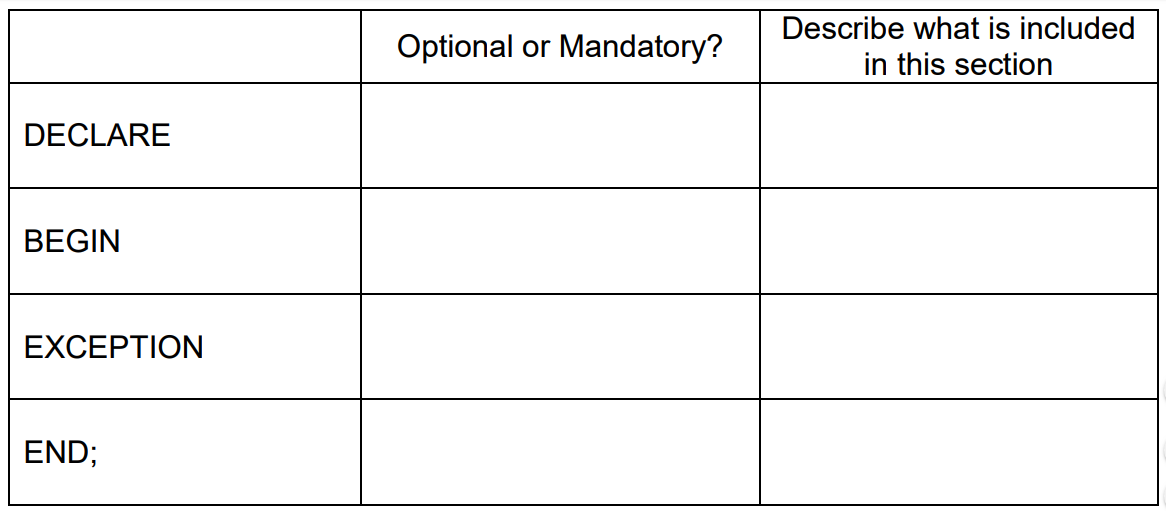
\includegraphics[width=15cm]{./Imagenes/actividad01}  
	\end{center}	

	   01.- DECLARE	= is optional -- 
	\\02.- BEGIN		= is Mandatory --
	\\03.- EXCEPTION	= is optional --
	\\04.- END		= is Mandatory --\\

	\subitem 02- Which of the following PL/SQL blocks executes successfully? For the blocks that fail, explain why they fail
	\\
	\subitem A. BEGIN
	\subitem    END;
	\subitem B. DECLARE
 	\subitem    amount INTEGER(10);
	\subitem    END;
	\subitem C. DECLARE
	 \subitem   BEGIN
	 \subitem   END;
	\subitem D. DECLARE
	 \subitem	amount NUMBER(10);
	 \subitem	begin
	 \subitem	DBMS\_OUTPUT.PUT\_LINE(amount);
	 \subitem	END;
	\\\\A.- ERROR ---------- FALTA EL EJECUTABLE
	\\B.-
	\\C.-
	\\D.- CORRECTO\\

	\subitem 03- Fill in the blanks:
	\subitem A. PL/SQL blocks that have no names are called \_\_\_\_\_\_\_\_\_\_\_\_\_\_\_\_\_\_.
	\subitem B. \_\_\_\_\_\_\_\_\_\_\_\_\_\_\_ and \_\_\_\_\_\_\_\_\_\_\_\_\_\_\_ are named blocks and are stored in the database.
	\\\\A.- ANONYMOUS BLOCKS
	\\B.- PROCEDURES --- FUNCTION

\end{enumerate}





\end{document}
